\chapter{Fundamentação Teórica}

Este capítulo tem como objetivo apresentar conceitos importantes para a
construção desta pesquisa e entendimento dos resultados obtidos. Assim, o capítulo abordará conceitos de metodologias ágeis, DevOps, técnicas de integração, entrega e \emph{deployment} contínuos e práticas relacionadas. Por fim, serão abordados alguns dos trabalhos relacionados a este.


\section{Metodologias Ágeis}

A citação a seguir retirada da dissertação \cite{experienciaComAgil} define bem os como os métodos ágeis surgiram.

    
\begin{quotation}[]{Dairton Luiz Bassi Filho}
    "Durante a evolução dos processos de Engenharia de Software, a
indústria se baseou nos métodos tradicionais de desenvolvimento de
software, que definiram por muitos anos os padrões para criação de
software nos meios acadêmico e empresarial. Porém, percebendo que a
indústria apresentava um grande número de casos de fracasso, alguns
líderes experientes adotaram modos de trabalho que se opunham aos
principais conceitos das metodologias tradicionais. Aos poucos, foram
percebendo que suas formas de trabalho, apesar de não seguirem os
padrões no mercado, eram bastante eficientes. Aplicando-as em vários 
projetos, elas foram aprimoradas e, em alguns casos, chegaram a se
transformar em novas metodologias de desenvolvimento de software.
Essas metodologias passaram a ser chamadas de leves por não
utilizarem as formalidades que caracterizavam os processos tradicionais
e por evitarem a burocracia imposta pela utilização excessiva de
documentos. Com o tempo, algumas delas ganharam destaque nos
ambientes empresarial e acadêmico, gerando grandes debates,
principalmente relacionados à confiabilidade dos processos e à
qualidade do software.
\end{quotation}

É notório que a antecipação total de requisitos, como propunha o modelo Cascata antigo, era a fórmula perfeita para a falha do projeto, como comenta \cite{agileSoftwareDevelopment}. Principalmente em ambientes de desenvolvimento de software, a metodologia mais interessante deve se basear em entregas parciais rápidas, com o objetivo de encontrar erros em fases iniciais e gerar um produto final mais de acordo com a expectativa do cliente. A ideia, como comenta o artigo, é reduzir o custo de mudanças durante o todo o desenvolvimento do projeto. As metodologias ágeis surgiram então com o objetivo de suprir essas necessidades.

No geral, é possível perceber que as metodologias ágeis conseguiram encantar as empresas de desenvolvimento de software principalmente por dar a habilidade de gerenciar mudanças de prioridades, ajudar no alinhamento entre as equipes de mercado e de tecnologia e aumentar a velocidade de entregas, de acordo com \cite{stateAgileReport2020}. Pesquisas como esta demonstram o sucesso que esse novo paradigma obteve no contexto de produção de aplicações de T.I. 

\vspace{3mm}
\subsection{SCRUM}
Uma das metodologias ágeis que apresenta uma grande quantidade de usuários é o SCRUM \cite{scrumBook}. Ele é um framework de gerenciamento de projetos que estabelece uma série de regras e cerimônias ao processo com o objetivo de garantir entregas iterativas e incrementais. Mesmo tendo sido criado em 1993 por Jeff Suntherland, a metodologia é - entre as ágeis - a mais utilizada atualmente: de acordo com a pesquisa da \emph{digital.ia} de 2020 \cite{stateAgileReport2020}, 58\% das equipes utilizam o framework na sua organização.

\begin{figure}[ht]
\begin{center}
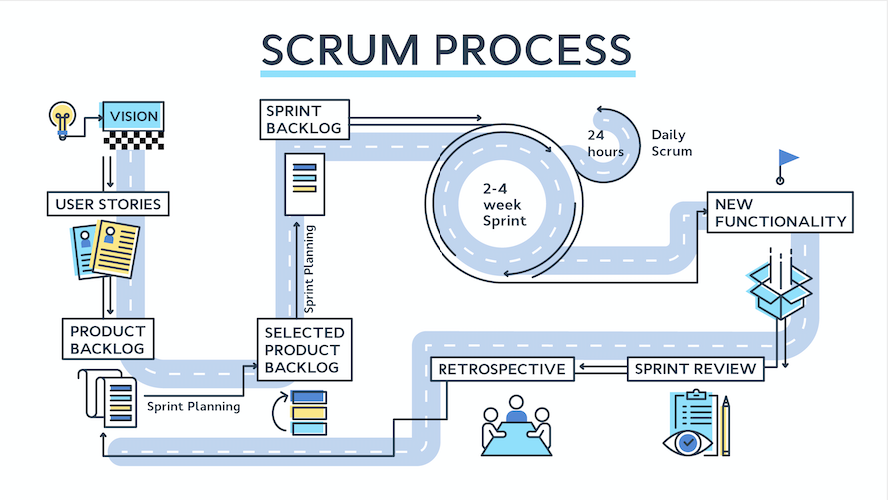
\includegraphics[width=\textwidth]{scrum.png}
\end{center}
\caption[O processo SCRUM]{
    O processo SCRUM. Fonte \cite{fotoScrum}
}\label{scrum}
\end{figure}

A \figref{scrum} mostra o processo da metodologia. No SCRUM, os ciclos de cada projetos são denominados \emph{Sprints}, que têm duração geralmente de uma semana e são planejados durante o \emph{Planning}. Esta reunião acontece no início da \emph{Sprint} e serve para decidir o conjunto de tarefas a ser feito pela equipe durante o tempo estipulado. As tarefas são retiradas do \emph{Backlog} do produto, que contém todos os objetivos e funcionalidades já acertados com o cliente que deverão ser feitos pela equipe.

Todos os dias acontece a chamada \emph{Daily meeting}: uma reunião diária para facilitar o acompanhamento do projeto, levantar discussão a respeito das atividades desenvolvidas para disseminar conhecimento e identificar possíveis impedimentos dentro da equipe. Estas reuniões, de acordo com o método, não devem durar mais do que 15 minutos, e, por este motivo, devem ser feitas em pé.

Ao final da \emph{Sprint} acontece a reunião de \emph{Review}, onde a equipe apresenta o que foi realizado durante a última iteração e os resultados do trabalho. Após ela, acontece também a cerimônia principal para garantia de melhoria contínua: a retrospectiva. Nela, a equipe discute melhorias que podem ser implementadas no processo para atingir uma velocidade maior de entregas.

Com a pesquisa da empresa \emph{digital.ia} \cite{stateAgileReport2020} é possível perceber que, mesmo não aplicando o SCRUM definido por Suntherland, várias das cerimônias definidas na metodologia são utilizadas: 85\% dos entrevistados fazem \emph{Daily's}, 81\% utilizam a cerimônia de retrospectiva e 77\%, \emph{Planning}. 

\section{DevOps}

Mesmo com a flexibilidade e agilidade das metodologias ágeis comentadas na seção anterior, as empresas ainda estavam necessitadas de um método de reduzir o tempo entre entregas de novas features. Esta foi a principal motivação para a criação da cultura de \emph{DevOps} \cite{devopsBook}. 

\begin{figure}[ht]
\begin{center}
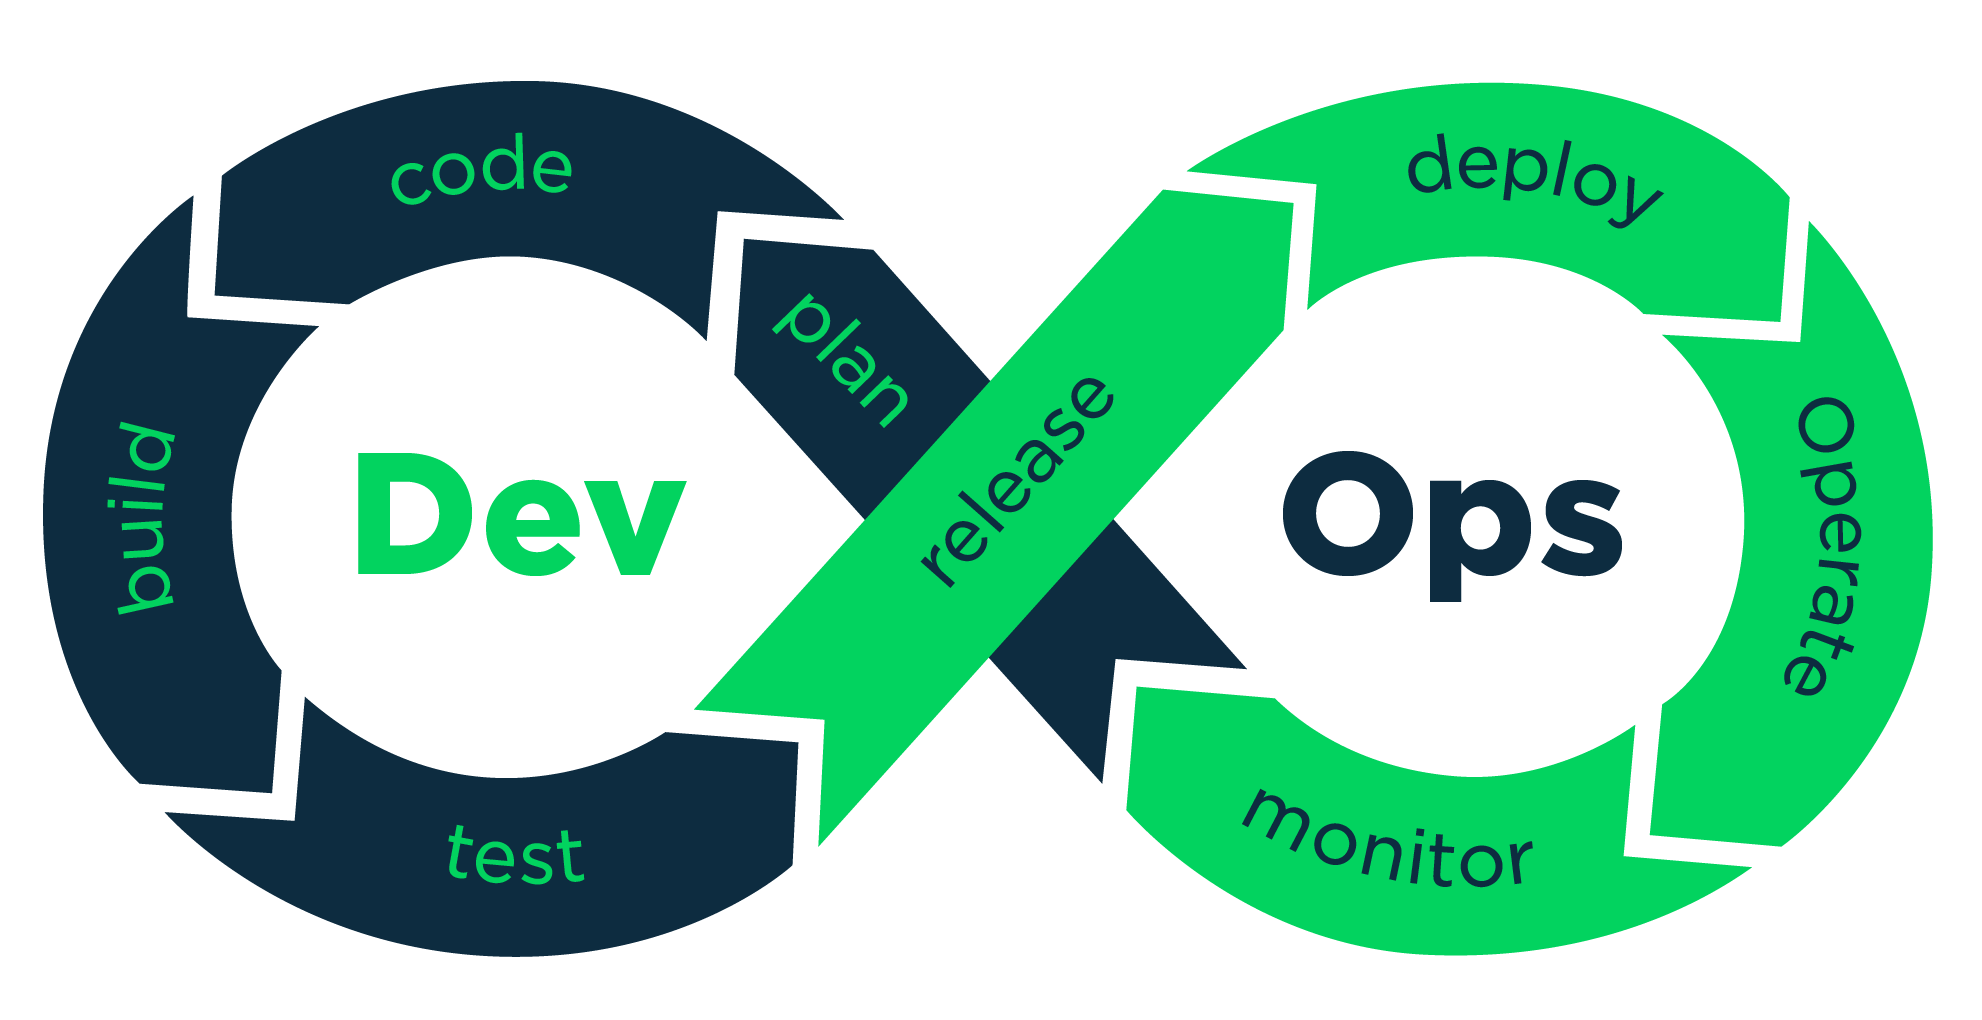
\includegraphics[scale=0.20]{devops.png}
\end{center}
\caption[A cultura DevOps]{
    A cultura DevOps
}\label{devops}
\end{figure}

\emph{DevOps} é definido como uma série de práticas que buscam reduzir o tempo entre a finalização de uma nova funcionalidade até que esta esteja em produção, garantindo ainda o máximo de qualidade da mesma. Mesmo contendo o tempo como uma das principais preocupações, é importante também para o método observar a importância da qualidade do que está sendo entregue em vários aspectos: segurança, disponibilidade, confiabilidade. Não adianta entregar funcionalidades rapidamente se essas não se comportam de acordo com o esperado ou expõem o software a ataques maliciosos.

Para atingir o seu objetivo, de acordo com \cite{devopsWiki}, a cultura de \emph{DevOps} prega a quebra de silos entre os desenvolvedores de software (Dev) e os administradores de sistema (Ops). Melhorar a comunicação entre os dois papéis e impulsionar a automação de processos e o monitoramento em todas as fases de desenvolvimento de um software auxiliam as empresas no gerenciamento de lançamento de novas versões e no processo de garantia de qualidade.

Dentre as práticas sugeridas pelo método, estão: \emph{Continuous Integration} (integração contínua);  \emph{Continuous Delivery} (entrega contínua) e \emph{Deployment}; e \emph{Partial Rollouts} (entregas parciais). Estas serão abordadas nas subseções seguintes.

\subsection{Integração Contínua}

A técnica de \emph{Continuous Integration} (integração contínua ou CI), de acordo com \cite{fowlerCI}, têm como principal característica a integração de código no repositório compartilhado múltiplas vezes por dia. Para garantir a qualidade do software que está sendo integrado, cada \emph{merge} passa por testes automáticos pré-programados que garantem que cenários de usabilidade estão de acordo com os requisitos definidos. 

Algumas práticas foram definidas dentro da técnica para definir processos chaves que produzem um CI eficiente. Entre elas, temos o \emph{trunk based development} \cite{devAndDeploymentFB}, onde todo o time contribui para uma única \emph{branch} no repositório de versionamento. Esta técnica é comumente utilizada para diminuir a quantidade de conflitos entre linhas de códigos que estão sendo concorrentemente modificadas por desenvolvedores diferentes. 

Para garantir que o \emph{trunk based development} funcione como esperado, deve-se ter uma ferramenta que possibilite o chaveamento de partes de código que ainda não foram finalizadas. A implementação comum desta técnica é \emph{feature toggle} \cite{featureToggles}. A técnica define, através de condicionais adicionadas no código fonte, que blocos devem ser executados ou ignorados no ambiente de produção.

Outra prática relacionada a técnica de integração contínua é o chamado \emph{developer awareness} \cite{awa}, que prega a quebra de silos entre os desenvolvedores e processos de \emph{release}, o status dos ambientes e informações gerais da infraestrutura do sistema que está sendo desenvolvido.

\subsection{Entrega e \emph{Deployment} Contínuos}

A técnica de \emph{Continuous Delivery} (entrega contínua ou CD) define que o software tem que estar a qualquer momento pronto para ser enviado para produção \cite{fowlerCD}. Para que a técnica de entrega contínua funcione como o esperado, é necessário principalmente que o software esteja pronto para \emph{deploy} durante todo o ciclo de vida e que o time sempre priorize deixar o código pronto para produção ao invés de priorizar novas funcionalidades.

Muitas vezes a técnica de \emph{Continuous Delivery} é confundida com a de \emph{Continuous Deployment}. No entanto, esta última significa que o código é automaticamente colocado em produção sempre que possível, resultando em múltiplos \emph{deployments} por dia. Com a entrega contínua, a empresa pode escolher ter um processo de entregas mais devagar, mesmo tendo o software sempre pronto para utilização. Outro ponto importante é que para se ter \emph{deployment} contínuo, é necessário ter entrega contínua.

A técnica de \emph{Continuous deployment} foi bastante difundida através do exemplo de empresas como a \emph{Flickr}, que em 2009 comentou sobre seus mais de 10 \emph{deploys} diários \cite{flickrTalk}, antes mesmo o termo \emph{DevOps} ser inventado. 

Algumas práticas definem alguns dos passos necessários para utilizar a técnica de CD. Podemos citar o \emph{deployment pipeline} \cite{devopsBook}, que define o conjunto de passos que qualquer mudança de código tem que passar para chegar em produção. Esses passos podem tratar da compilação do código, da execução de testes em diferentes ambientes, entre outras coisas e pode ser totalmente ou parcialmente automatizada.

Depois da entrega de uma nova versão, \emph{health checks} \cite{devopsBook} são necessários para garantir que o produto está funcionando corretamente. O sistema tem uma série de parâmetros definidos pela equipe que mostram se há algum problema no ambiente de produção, por exemplo, falha na conexão com o banco de dados, serviços inativos, certificados HTTPS expirados, entre outros. Muitas vezes o sistema tem a funcionalidade de envio de mensagens para os responsáveis quando algo de errado ocorre no ambiente.

Para garantir ainda mais uma colaboração maior entre desenvolvedores e o time de operações, surgiu a prática de \emph{developer on call} \cite{devAndDeploymentFB}. Esta sugere que o desenvolvedor responsável pela funcionalidade recém lançada fique disponível por tempo extra após o lançamento em produção. Caso haja algum erro, ele será a pessoa mais propícia a resolvê-lo o mais rápido possível.

\subsection{Entregas Parciais}
A prática de \emph{partial rollouts} (ou entregas parciais) pode ser definida como um processo de garantia de qualidade e validação de requisitos que ocorrem em tempo de execução \cite{empiricalStudy2016}. Dentre as técnicas ligadas, podemos citar \emph{canary releases} \cite{continuousDeliveryBook}, que define o ato de enviar versões apenas para uma parte dos usuários ativos. Isto serve para testar mudanças no software primeiramente com uma parcela pequena de clientes.

Outra prática relacionada a técnica é a de Testes A/B \cite{testsAB}. Ela se baseia no teste concorrente de duas ou mais versões rodando paralelamente, que se diferem em um ponto isolado do sistema. A ideia é avaliar através de medidas estatísticas de uso e performance do sistema quais das versões é a mais pertinente aos requisitos do software. O teste pode mostrar desde versões que representam um tempo de resposta mais rápido para o usuário, até o lugar que um botão deve aparecer para vender mais produtos.

A prática de \emph{dark launches} \cite{devAndDeploymentFB} também se enquadra dentro das técnicas de entregas parciais. Ela é utilizada para testes de funcionalidades no ambiente de produção, mas sem a necessidade de habilitar a mesma para os usuários. Geralmente é utilizado para testar excentricidades encontradas especificamente apenas em produção.  


\section{Code Review}

A técnica de \emph{code review} \cite{codeReview} consiste em uma inspeção manual das mudanças por desenvolvedores diferentes daquele responsável pelo desenvolvimento da mudança. Esta é uma técnica utilizada desde projetos Open Source até softwares industriais. Serve principalmente como forma de compartilhar conhecimento e fomentar discussões produtivas a respeito de soluções produzidas pela equipe.

\section{Trabalhos Relacionados}

Há vários trabalhos relacionados a benefícios e barreiras que existem na adoção de integração contínua em contextos variados. É possível perceber que no geral os desenvolvedores gostam de utilizar CI por garantir um desenvolvimento de uma forma mais segura e confiável \cite{googleCi} e por se sentirem mais produtivos \cite{hilton2016}. É possível perceber também que os desenvolvedores ainda acham que as ferramentas de CI são complicadas e difíceis de configurar \cite{hilton2016}. 

É interessante levantar ainda no contexto de integração contínua que utilizar as ferramentas voltadas para esta técnica sem adequar a cultura de desenvolvimento para tal leva a práticas não saudáveis de desenvolvimento, tais como \emph{builds} que levam muito tempo para concluir ou permanecem quebrados por longos períodos de tempo  \cite{citheater2019}. Outro estudo encontrou que a utilização da técnica apresenta um \emph{trade-off} entre velocidade e certeza no que diz respeito a garantia de qualidade do software \cite{hilton2016}.

Já a respeito de \emph{deployment} contínuo, foi encontrada a visão dos desenvolvedores do Facebook e de OANDA a respeito desta técnica \cite{savor2015}. O artigo mostra que os desenvolvedores preferem \emph{deployments} mais rápidos por gerar maior qualidade de software e maior produtividade. Contudo, eles acreditam que há uma instabilidade maior e é uma metodologia inviável para sistemas críticos.

Podemos ainda citar o artigo mais relacionado e que também serve de base para este trabalho \cite{empiricalStudy2016}, que apresenta uma pesquisa empírica a respeito dos princípios e práticas de entrega e \emph{deployment} contínuos em empresas européias e norte-americanas. Os autores encontram que umas das principais barreiras para a adoção de CD são problemas arquiteturais. Além disso, percebe-se que \emph{feature toggles} como uma implementação de técnicas de entregas parciais levam a uma complexidade de código indesejada.
